%%%%%%%%%%%%%%%%%%%%%%%%%%%%%%%%%%%%%%%%%%%%%%%%%%%%%%%%%%%%%%%%
\section{Hybrid Co-Simulation Algorithm}
\label{sec:impl_hybrid}

The previous sections described the master algorithms and the structural metadata used during macro-step execution.
This section extends that implementation to hybrid co-simulation and realizes the concepts introduced in Section~\ref{sec:236_cosim_hybrid}.
It addresses SR-10-04 under UR-10 in Table~\ref{tab:req_simulation}, which requires system-level detection, localization, and propagation of discrete events across coupled subsystem models.
The hybrid orchestration is implemented as \texttt{HybridAlgorithm} and reuses \texttt{GaussSeidelAlgorithm} as the continuous algorithm, between events.
It also relies on the hybrid component hooks and event connections introduced in Sections~\ref{sec:impl_component_interface} and~\ref{sec:impl_system}.

%%%%%%%%%%%%%%%%%%%%%%%%%%%%%%%%%%%%%%%%%%%%%%%%%%%%%%
\subsection{Scope and Component Contract}
\label{sec:impl_hybrid_scope}

Hybrid execution is activated during \texttt{System.initialize(t0)}.
The system classifies the registered components into event sources, event listeners, and continuous-only components.
If at least one event source is present, the selected algorithm is replaced by \texttt{HybridAlgorithm}.
Otherwise, the continuous execution path remains unchanged.

A component becomes an event source by registering an indicator with \pyfn{add\_event\_indicator()}.
The resulting \texttt{EventIndicator} stores the scalar indicator function and the crossing direction.
Rollback support is required because event detection and localization use trial steps inside a macro step.
This requirement is enforced through \texttt{supports\_rollback} when the indicator is registered.
A component becomes an event listener when an \texttt{EventConnection} subscribes it to an event produced by another component.

Event times are stored as \texttt{DenseTime} objects.
Each object combines the physical time $t$ with a microstep index $\nu$.
This allows the algorithm to order cascaded events that occur at the same physical time.

Table~\ref{tab:hybrid_component_contract} summarizes the hybrid-specific operations used by \texttt{HybridAlgorithm}.
The general component interface is described in Section~\ref{sec:impl_component_interface}.

\begin{table}[htbp]
  \centering
  \caption{Hybrid component operations used by \texttt{HybridAlgorithm}.}
  \label{tab:hybrid_component_contract}
  \begin{tabular}{lp{10cm}}
    \toprule
    \textbf{Operation} & \textbf{Role in hybrid execution} \\
    \midrule
    \texttt{evaluate\_event\_indicators()} & Returns the current indicator values \\
    \texttt{detect\_event\_crossings()} & Detects crossings between two indicator states \\
    \texttt{snapshot\_state()} & Captures the rollback state before a trial step \\
    \texttt{restore\_state()} & Restores the component after trial stepping or bisection \\
    \texttt{handle\_event()} & Applies event-driven state updates \\
    \texttt{report\_internal\_event()} & Reports optional event brackets from internal micro-stepping \\
    \bottomrule
  \end{tabular}
\end{table}

Event routing is stored on the \texttt{System}.
During \pyfn{add\_event\_connection()}, each \pyfn{EventConnection} adds one source-event to listener mapping to \pyfn{\_event\_targets\_by\_source}.
The hybrid algorithm queries this mapping when localized events are dispatched.

%%%%%%%%%%%%%%%%%%%%%%%%%%%%%%%%%%%%%%%%%%%%%%%%%%%%%%
\subsection{Hybrid Macro-Step Sequence}
\label{sec:impl_hybrid_macro_step}

The entry point of the hybrid algorithm is \texttt{step(system, t, dt)}.
The method advances the system from the current communication time $t$ to $t + \Delta t$ and stores the interval boundaries as \texttt{t\_left} and \texttt{t\_right}.
An outer while loop iterates over \texttt{t\_left} so that one invocation of \texttt{step()} may internally resolve several events at different times in the interval.
Figure~\ref{fig:impl_hybrid_macro_step} summarizes the five phases of one outer iteration.

\begin{figure}[t]
    \centering
    \includegraphics[width=0.85\linewidth]{diagrams/out/pdf/execution/hybrid/Hybrid_Step.pdf}
    \caption{Implementation-level macro-step orchestration of the hybrid co-simulation algorithm.
    Each interval starts with input preparation and trial event detection.
    If no crossing is found, the remaining interval is advanced by the Gauss--Seidel path.
    If a crossing is found, the event time is localized, the system is advanced to that time, and event handling is iterated in superdense time until no further cascaded event remains.}
    \label{fig:impl_hybrid_macro_step}
\end{figure}

At each new value of \texttt{t\_left}, \texttt{\_prepare\_inputs()} propagates the current signal values generation by generation.
If a generation contains an algebraic loop, the local SCC solver from Section~\ref{sec:impl_algebraic_loops} is applied before event detection continues.
The algorithm then performs the trial-step-based detection described in Section~\ref{sec:impl_hybrid_detection} for every registered event source in the interval \texttt{[t\_left, t\_right]}.

If no crossing is found, the remaining interval is handled as a continuous co-simulation step.
The algorithm delegates this part to \texttt{GaussSeidelAlgorithm.step()} and returns.
Hybrid execution therefore has the same continuous stepping behavior as the Gauss--Seidel algorithm as long as no event interrupts the macro step.

If a crossing is found, the algorithm localizes the event time \texttt{t\_event} inside the current interval and advances the full coupled system only up to that time.
The detected events are recorded with their \texttt{DenseTime} stamps and dispatched to the subscribed listeners.
Event handlers may update component states, so \texttt{\_prepare\_inputs()} is called again and the algorithm checks whether the handling has triggered further events at the same physical time.
Event detection, event time localization, and the iterative event handling are described in Sections~\ref{sec:impl_hybrid_detection}, \ref{sec:impl_hybrid_localization}, and~\ref{sec:impl_hybrid_handling}.
The outer iteration concludes once no further event is pending at the current physical time.
The remaining part of the original macro step is then processed by the same loop.

%%%%%%%%%%%%%%%%%%%%%%%%%%%%%%%%%%%%%%%%%%%%%%%%%%%%%%
\subsection{Event Detection via Trial Stepping}
\label{sec:impl_hybrid_detection}

Event detection is implemented in \texttt{\_detect\_crossings()}.
For each event source, the algorithm first stores a rollback snapshot and caches the current input port values.
It then evaluates the event indicators at the left interval boundary.
After this, the component is advanced in a trial step to the right interval boundary and its indicators are evaluated again.
The two indicator vectors are passed to \texttt{detect\_event\_crossings()}, which applies the registered crossing directions of the event indicators.

The trial step must not change the accepted simulation state.
Therefore, the component is restored to the left boundary after its indicators and optional internal event hints have been collected.
Detection is a single pass over all event sources and collects the detected crossing names together with any \texttt{InternalEventInfo} hints supplied by the source.
Only the detected crossing names and the event brackets are kept by the algorithm.

\subsection{Event Time Localization}
\label{sec:impl_hybrid_localization}

If at least one crossing was detected, \texttt{\_locate\_event\_time()} searches for the earliest event time in the interval.
The implementation uses bisection between the current left and right boundaries.
At each candidate time, the event sources are restored to the left boundary, advanced to the candidate time, and evaluated again.
The interval is narrowed until its width is below \texttt{tol\_time} or the indicator magnitude at the midpoint is below \texttt{tol\_value}.

Components with internal micro-stepping may report event brackets through \pyfn{report\_internal\_event()}.
Each bracket is an \pyfn{InternalEventInfo} instance with the fields \pyfn{event\_name}, \texttt{t\_before}, and \texttt{t\_after}, optionally accompanied by the indicator values at those two times.
The hybrid algorithm consumes these brackets through \pyfn{get\_internal\_event\_hints()} and uses the earliest valid hint to narrow the initial bisection interval.
This does not change the event handling semantics.
It only reduces the localization interval when the component can provide more precise internal timing information.

After localization, the algorithm evaluates the indicators once more at the located time and collects all events that are active there.
It then restores every event source to \texttt{t\_left} so the next phase can advance the full coupled system to \texttt{t\_event} through the main macro-step sequence.
Detection and localization therefore leave the accepted simulation state untouched.

%%%%%%%%%%%%%%%%%%%%%%%%%%%%%%%%%%%%%%%%%%%%%%%%%%%%%%
\subsection{Event Handling at Dense Time}
\label{sec:impl_hybrid_handling}

Once the localized event time \texttt{t\_event} has been returned to the main macro-step sequence, the hybrid algorithm advances the full coupled system to that time through \pyfn{GaussSeidelAlgorithm.step(system, t\_left, t\_event - t\_left)}.
This is a shortened continuous step that uses the same orchestration as every other continuous advance.

Before the handlers run, the algorithm filters the event list against a per-step cache of already-handled events.
Two events at the same component are treated as duplicates when their physical times differ by less than \texttt{event\_dedup\_tol}.
The cache is cleared at the beginning of each call to \texttt{step()} and prevents the same crossing from being handled twice across consecutive outer iterations.

Event handling proceeds in an inner loop that supports cascaded events at the same physical time.
The iteration advances the microstep index $\nu$ of \texttt{DenseTime} and terminates once no further event is triggered.
Each iteration first records the pending events in the system history and takes a before-handling snapshot of the event indicators.
It then dispatches the events through \texttt{handle\_events()}, re-prepares the component inputs, and evaluates the indicators again.
Cascaded events are the crossings between the before-handling and the after-handling indicator vectors.
If the iteration produces such events, the microstep index is advanced through \texttt{DenseTime.advance\_micro()} and the loop continues with the new event list.
The safeguard \texttt{max\_microsteps} aborts the iteration with a runtime error if the loop fails to converge.

The dispatch method \texttt{handle\_events()} groups pending events by listener component.
If a listener receives more than one event at the same dense time, the algorithm verifies that the handlers commute.
An annotation-based check is attempted first through \texttt{event\_commutativity}, which records pairwise commutativity known to the component.
If no annotation is available, a dynamic check runs all handler permutations from a shared snapshot and compares the resulting states through \texttt{\_states\_equal()}.
A non-commutative event set raises a runtime error rather than committing a non-deterministic result.
Commuting handlers are then dispatched one by one through \texttt{System.dispatch\_event()}.

After the inner loop terminates, the algorithm re-prepares the inputs once more and advances \texttt{t\_left} to \texttt{t\_event} plus \texttt{tol\_time}.
This small offset prevents the same crossing from being re-detected in the next outer iteration.
The main macro-step loop then processes the remaining interval \texttt{[t\_left, t\_right]} under the same scheme.

\subsection{Verification}

\paragraph{Event chain and superdense time.}
The first scenario verifies the superdense microstep loop through a three-component event chain.
A \texttt{HybridSource} with $x_{\mathrm{src}}(t) = -\tfrac{2}{3} + 2\,t$ emits a zero-crossing event at the analytical time $t_e = \tfrac{1}{3}\,$s.
The event is routed to a \texttt{HybridCombi} that reacts by doubling its velocity from $-1$ to $-2$.
The velocity change is itself an event indicator on the \texttt{HybridCombi} and produces a second event at the same physical time.
This cascaded event is routed to a \texttt{HybridListener} that inverts its velocity from $+3$ to $-3$.
The algorithm should therefore locate both events at the same physical time but at different microstep indices, namely $(t_e, 0)$ and $(t_e, 1)$.

Figure~\ref{fig:impl_hybrid_verification_chain} shows the state trajectories of the three components together with the located event time.
The algorithm detects the zero-crossing of the \texttt{HybridSource} in the macro interval $[0.30, 0.35]\,$s and locates the event at $t_e \approx 0.33333359\,$s.
The first handler doubles the \texttt{HybridCombi} velocity at microstep~$0$ and the cascaded-event check detects the induced velocity change at the same physical time.
The second handler then inverts the \texttt{HybridListener} velocity at microstep~$1$.
The post-event slopes of the Combi and Listener trajectories match the analytical post-event dynamics with $v_{\mathrm{combi}} = -2$ and $v_{\mathrm{lis}} = -3$.
The located event time agrees with the analytical value $t_e = 1/3\,$s within the indicator tolerance \texttt{tol\_value}, with an observed absolute error of about $2.6\cdot 10^{-7}\,$s.

\begin{figure}[!htbp]
    \centering
    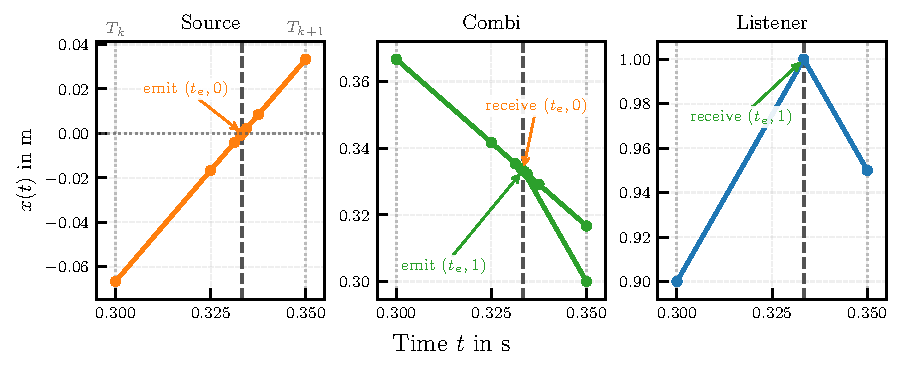
\includegraphics[width=\linewidth]{figures/5_implementation/hybrid/hybrid_event_chain.pdf}
    \caption{Event chain resolved with superdense time.
    The light dotted lines mark the original communication interval from $T_k = 0.30\,$s to $T_{k+1} = 0.35\,$s.
    The dark dashed line marks the localized event time inserted by the hybrid algorithm.
    The source emits the first event at $(t_e,0)$.
    The Combi component handles this event and emits a cascaded event at $(t_e,1)$.
    The Listener receives the cascaded event at the same physical time.}
    \label{fig:impl_hybrid_verification_chain}
\end{figure}

\paragraph{Strong event simultaneity and commutativity.}
The second scenario verifies the commutativity check that activates when two events reach the same listener at the same dense time.
Two \texttt{HybridSource} components are configured so that their zero-crossings coincide at the analytical time $t_e = \tfrac{2}{3}\,$s.
\texttt{Source\_1} has $x_1(t) = \tfrac{2}{3} - t$ with falling-edge direction.
\texttt{Source\_2} has $x_2(t) = -\tfrac{2}{3} + t$ with rising-edge direction.

A single \texttt{HybridListener} with initial velocity $v_0 = 3.0\,$m/s subscribes to both events and applies the updates $v \mapsto -v$ and $v \mapsto 2v$.
The two updates commute, so the final velocity must equal $-2\,v_0$ regardless of the dispatch order.

Figure~\ref{fig:impl_hybrid_verification_simultaneity} shows the located event time and the resulting listener trajectory.
The algorithm detects both crossings in the macro interval from $0.65$ to $0.70\,$s and locates them at the dense time $(t_e, 0)$ with $t_e \approx 0.66666667\,$s.
The post-event listener velocity is $-6.0\,$m/s, which matches the expected value $-2\,v_0$.

Listing~\ref{lst:hybrid_simultaneity_log} documents the commutativity dispatch.
Both events are grouped on the \texttt{Listener} and trigger a dynamic commutativity check because the listener does not declare commutativity through an annotation.
The check runs both handler permutations from a shared snapshot and confirms identical final states.
Both events are then dispatched at microstep $0$ through \texttt{System.dispatch\_event()}.

\begin{figure}[t]
    \centering
    \begin{subfigure}[t]{0.48\linewidth}
        \centering
        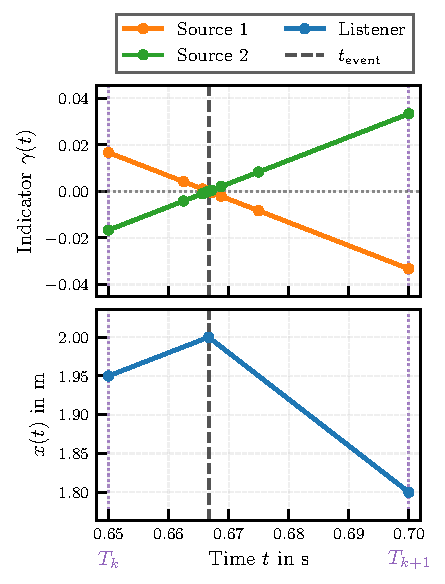
\includegraphics[width=\linewidth]{figures/5_implementation/hybrid/strong_simultaneity.pdf}
        \caption{Strong event simultaneity. Both sources cross zero at the same dense time $(t_e, 0)$ and the listener velocity is updated through commutative handlers.}
        \label{fig:impl_hybrid_verification_simultaneity}
    \end{subfigure}
    \hfill
    \begin{subfigure}[t]{0.48\linewidth}
        \centering
        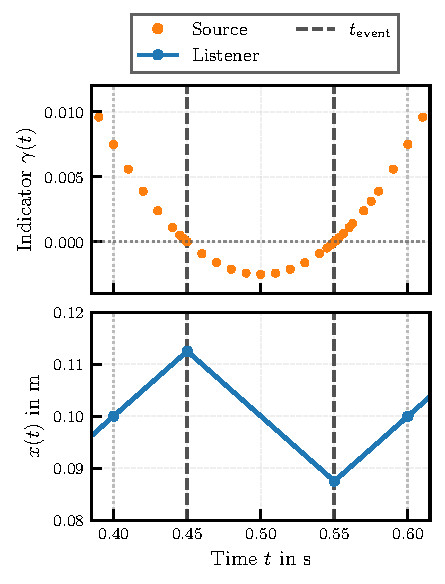
\includegraphics[width=\linewidth]{figures/5_implementation/hybrid/internal_event_reporting.pdf}
        \caption{Internal event reporting. The events at $t = 0.45\,$s and $t = 0.55\,$s lie strictly inside the macro interval $[0.4, 0.6]\,$s and are localized through internal hints.}
        \label{fig:impl_hybrid_verification_internal}
    \end{subfigure}
    \caption{Verification scenarios for two hybrid features that are not exercised in the case study. Dashed gray lines mark the localized event times; dotted gray lines mark the macro communication grid.}
    \label{fig:impl_hybrid_verification_pair}
\end{figure}


\begin{listing}[!htbp]
\begin{lstlisting}[
    basicstyle=\ttfamily\footnotesize,
    frame=single,
    backgroundcolor=\color{black!3},
    breaklines=true,
    columns=fullflexible,
    xleftmargin=0pt
]
Event crossing in [0.650000, 0.700000]: Source_1.v_invert, Source_2.v_double
Event located at t=0.66666667
Handling 2 event(s) at t=0.66666667, micro=0: Source_1.v_invert, Source_2.v_double
Events grouped by listener: {'Listener': ['v_invert', 'v_double']}
Checking commutativity for ['v_invert', 'v_double'] on Listener
Verifying commutativity dynamically for ['v_invert', 'v_double'] on Listener
Commutativity verified (dynamic): ['v_invert', 'v_double'] on Listener
\end{lstlisting}
\caption{Hybrid algorithm log for the strong-simultaneity scenario. Both crossings are localized at the same dense time, grouped on the listener, and confirmed commutative through the dynamic check before dispatch.}
\label{lst:hybrid_simultaneity_log}
\end{listing}

\paragraph{Internal event reporting.}
The third scenario verifies the internal-hint mechanism that allows components with internal micro-stepping to expose events between communication points.
An \texttt{EventReportingComponent} carries the indicator $h(t) = (t - T_1)(t - T_2)$ with roots $T_1 = 0.45\,$s and $T_2 = 0.55\,$s.
It steps internally with $\Delta t_{\mathrm{int}} = 0.01\,$s and reports an \texttt{InternalEventInfo} bracket whenever $h$ changes sign between two micro-steps.
An \texttt{EventListener} subscribes to the resulting \texttt{zero\_crossing} event and inverts its slope on every reception.
The macro step is set to $\Delta t = 0.2\,$s so that both roots fall strictly inside one macro interval.

The macro communication points alone cannot detect these events.
At both endpoints of the interval $[0.4, 0.6]\,$s the indicator is positive with $h(0.4) = h(0.6) = 0.0075$, so the trial-step detection of Section~\ref{sec:impl_hybrid_detection} would see no sign change.
The internal-hint mechanism resolves this by exposing the brackets $[0.44, 0.45]\,$s and $[0.54, 0.55]\,$s that the component records during its micro-steps.

Figure~\ref{fig:impl_hybrid_verification_internal} shows the indicator and the listener trajectory together with the macro grid.
The first hint narrows the bisection to $[0.44, 0.45]\,$s and the event is located at $t = 0.45\,$s.
The handler inverts the listener slope.
The second hint then narrows the bisection to $[0.54, 0.55]\,$s and the second event is located at $t = 0.55\,$s.
The two located event times agree with the analytical roots $T_1$ and $T_2$ within machine precision.

After the second event, a residual trial-step detection on $[0.55, 0.60]\,$s reports a rising crossing because the indicator at the new left boundary is below the sign tolerance.
The per-step deduplication cache rejects this detection since the time difference to the previously handled event is below \texttt{event\_dedup\_tol}.